\documentclass[xcolor=table,      handout ,    xcolor=dvipsnames]{beamer}\usepackage[]{graphicx}\usepackage[]{color}
% maxwidth is the original width if it is less than linewidth
% otherwise use linewidth (to make sure the graphics do not exceed the margin)
\makeatletter
\def\maxwidth{ %
  \ifdim\Gin@nat@width>\linewidth
    \linewidth
  \else
    \Gin@nat@width
  \fi
}
\makeatother


\definecolor{fgcolor}{rgb}{0, 0, 0}
\newcommand{\hlnum}[1]{\textcolor[rgb]{0,0,0}{#1}}
\newcommand{\hlstr}[1]{\textcolor[rgb]{0.545,0.137,0.137}{#1}}
\newcommand{\hlcom}[1]{\textcolor[rgb]{0,0.392,0}{\textit{#1}}}
\newcommand{\hlopt}[1]{\textcolor[rgb]{0,0,0}{#1}}
\newcommand{\hlstd}[1]{\textcolor[rgb]{0,0,0}{#1}}
\newcommand{\hlkwa}[1]{\textcolor[rgb]{1,0,0}{\textbf{#1}}}
\newcommand{\hlkwb}[1]{\textcolor[rgb]{0,0,0}{#1}}
\newcommand{\hlkwc}[1]{\textcolor[rgb]{1,0,1}{#1}}
\newcommand{\hlkwd}[1]{\textcolor[rgb]{0,0,1}{#1}}


\usepackage{framed}
\makeatletter
\newenvironment{kframe}{%
 \def\at@end@of@kframe{}%
 \ifinner\ifhmode%
  \def\at@end@of@kframe{\end{minipage}}%
  \begin{minipage}{\columnwidth}%
 \fi\fi%
 \def\FrameCommand##1{\hskip\@totalleftmargin \hskip-\fboxsep
 \colorbox{shadecolor}{##1}\hskip-\fboxsep
     % There is no \\@totalrightmargin, so:
     \hskip-\linewidth \hskip-\@totalleftmargin \hskip\columnwidth}%
 \MakeFramed {\advance\hsize-\width
   \@totalleftmargin\z@ \linewidth\hsize
   \@setminipage}}%
 {\par\unskip\endMakeFramed%
 \at@end@of@kframe}
\makeatother

\definecolor{shadecolor}{rgb}{.97, .97, .97}
\definecolor{messagecolor}{rgb}{0, 0, 0}
\definecolor{warningcolor}{rgb}{1, 0, 1}
\definecolor{errorcolor}{rgb}{1, 0, 0}
\newenvironment{knitrout}{}{} % an empty environment to be redefined in TeX

\usepackage{alltt} % , handout, draft
\usetheme{Madrid} % Madrid, Warsaw, Berlin
\usecolortheme{beaver}

\usepackage[latin1]{inputenc} % windows
%\usepackage[utf8]{inputenc} %linux
\usepackage[T1]{fontenc} % for textbackslash
\usepackage[german, english]{babel}
\usepackage{float} % placing floats (table and figures) where they should be
\usepackage{lmodern} % make tiny font shape warnings within the beamer class diappear
\usepackage{tabu, multirow, url, hyperref, textcomp, amsmath, listings, datetime, graphicx, booktabs, xcolor, multicol, setspace}
\usepackage[absolute,overlay,showboxes]{textpos}
\usepackage{wasysym}
\usepackage{fontawesome}

\hypersetup{pdfstartview={XYZ null null 1}}
\hypersetup{colorlinks=true, linkcolor=blue, urlcolor=blue}

\setbeamertemplate{footline}[text line]{%
  \parbox{\linewidth}{\vspace*{-8pt}
  \href{https://github.com/brry/course\#slides}{github.com/brry/course} \hfill
  \hyperlink{toc}{TOC} ~~ \insertframenumber / \inserttotalframenumber~~~~~~~~~}}
\setbeamertemplate{navigation symbols}[only frame symbol]

\beamersetleftmargin{0.3cm}
\beamersetrightmargin{0.3cm}

% Reduce spacing in table of contents (toc) http://tex.stackexchange.com/questions/51452
\usepackage{etoolbox}
\makeatletter
\patchcmd{\beamer@sectionintoc}{\vskip1.5em}{\vskip0.1em}{}{} % vskip0.5em
\makeatother

% Remove Bullets and Numbers in TOC: http://tex.stackexchange.com/questions/54656
\setbeamertemplate{sections/subsections in toc}[default]

% white letters in enumerate bullet points
%\definecolor{stupidblue}{RGB}{51,51,178}
\setbeamercolor{item projected}{fg=white}%fg=blue,bg=red!75!black} % fg=white , bg=stupidblue
\setbeamercolor{frametitle}{fg=black}
% Block title color
\setbeamercolor{block title}{fg=white}%fg=blue,bg=red!75!black} % white
%\setbeamertemplate{item projected}[square]


% define an environment for the exercises
\newcounter{exercisecount}
\setcounter{exercisecount}{0}
\newenvironment{exercise}[1]
{% This is the begin code
\stepcounter{exercisecount}
\begin{block}{Exercise \arabic{exercisecount}: #1}
}
{% This is the end code
\end{block} }

\resetcounteronoverlays{exercisecount}

% format inline R command names in blue courier and lightgrey background:
\newcommand{\rcode}[1]{\texttt{\textcolor{Blue}{#1}}}
\newcommand{\key}[1]{\colorbox{gray!30}{\texttt{\textcolor{Blue}{#1}}}}


% links to files
\newcommand{\datalinkRaw}[1]{\href{https://raw.githubusercontent.com/brry/course/master/data/#1}{#1}}
\newcommand{\datalinkBlob}[1]{\href{https://github.com/brry/course/blob/master/data/#1}{#1}}
\newcommand{\datalinkText}[1]{\href{https://github.com/brry/course/blob/master/data/#1}{#1} 
                            {\footnotesize \textit{(rightclick \textbf{Raw}, save as)}}}
                           
% Format month with leading zero:
\newcommand{\leadingzero}[1]{\ifnum #1<10 0\the#1\else\the#1\fi}

% "#' " for doc files:
\newcommand{\doc}{\#\textquotesingle~}

% remove empty lines between code and output. apparently hard to get rid of without turning off syntax highlighting


%------------------------------------------------------------%
%------------------------------------------------------------%
\IfFileExists{upquote.sty}{\usepackage{upquote}}{}
\begin{document}
%------------------------------------------------------------%
%------------------------------------------------------------%

\AtBeginSection[]
{
\begin{frame}%[shrink]
{Outline}
\scriptsize
\tableofcontents[sectionstyle=show/shaded, subsectionstyle=show/shaded/hide]
\end{frame}
}

%\def\newblock{}	% beamer---natbib bugfix






{\usebackgroundtemplate{
\includegraphics[width=\paperwidth]{fig/slidebg-1.pdf}}
\begin{frame}
\begin{center}
    \begin{columns}
    \column{15em}
    \begin{block}{}{\Large ~loops and functions in~ 
\includegraphics[width=0.7cm]{externalfig/Rlogo.png}}
    \end{block}
    \end{columns}
\vspace{1em}
Berry Boessenkool, \texttt{berry-b@gmx.de}\\
Jannes Breier, \texttt{jbreier@gfz-potsdam.de}\\[1em]
These slides and tasks are a subset of Berry's teaching material at\\
\href{https://github.com/brry/course}{github.com/brry/course}\\[1em]
These slides are licenced under
\href{https://creativecommons.org/licenses/by/4.0}{
\includegraphics[width=3em]{externalfig/ccby.png}},\\
so you can use the material freely as long as you cite us.\\[1em]
R installation instructions: \href{https://github.com/brry/course\#install}{github.com/brry/course\#install}\\[2em]
\scriptsize
PDF created on \the\year-\leadingzero{\month}-\leadingzero{\day}, \currenttime\ \\[1em]
\end{center}
\end{frame}
}

%------------------------------------------------------------%

\begin{frame}{Outline}
%%%\hspace{0.9em} \hyperlink{titlepage}{R course Info}\\[0.4em]
\tableofcontents[hideallsubsections]
\label{toc}
\end{frame}

%------------------------------------------------------------%

\begin{frame}{\rcode{print("Hello world!")}}
\begin{itemize}[<+->]
\item Berry Boessenkool $\rightarrow$ Geoecology @ Potsdam University
\item R Fan\onslide<+->atic \onslide<+-> since 2010
\item Developer of \href{https://github.com/brry/rdwd\#rdwd}{\texttt{rdwd}},
 \onslide<+-> Freelance trainer \& consultant \href{https://brry.github.io}{
\includegraphics[width=0.5cm]{externalfig/Blogo.png}}\\[1em]
\item Jannes Breier $\rightarrow$ Geoecology @ Potsdam University
\item Berry taught me R in 2013 \smiley{}
\item \href{https://www.linkedin.com/in/jbreier/}{\faLinkedinSquare} Research Software Engineer at GFZ, \href{https://www.gfz-potsdam.de/en/staff/jannes-breier/sec44/}{
\includegraphics[width=0.65cm]{externalfig/GFZ.png}} Sec.4.4: Hydrology \\[1em]
\item \alert{If we're proceeding too fast, please interrupt!}
\end{itemize}
\end{frame}

\iffalse % commenting out Conditions section
%------------------------------------------------------------%
%------------------------------------------------------------%
\section{Conditions}
%------------------------------------------------------------%
%------------------------------------------------------------%

\begin{frame}[fragile]{Conditional execution I}
Syntax for a single logical value:\\
\rcode{\alert{if}(this\_is\_true) \{do\_something\} \alert{else} \{do\_other\_thing\}}\\[\baselineskip]
\pause
Syntax for a vector with several T/F values:\\
\rcode{\alert{ifelse}(condition, expression1, expression2)}\\[\baselineskip]
\pause
If condition == TRUE, then expression1 is evaluated,
if condition == FALSE, then expression2 is evaluated.\\[1em]
\pause
\begin{columns}
\begin{column}{.40\textwidth}
\texttt{7-3 > 2 \\
\textcolor{blue}{class}(7-3 > 2 ) \\
\textcolor{red}{if}(7-3 > 2) 18  \\
\textcolor{red}{if}(7-3 > 5) 18  \\
\textcolor{red}{if}(7-3 > 5) 18 \textcolor{red}{else} 17 }
\end{column}
\begin{column}{.59\textwidth}
\pause TRUE\\
\pause logical = truth value, boolean\\
\pause Condition is TRUE, so 18 is returned\\
\pause Condition is FALSE, so nothing happens\\
\pause Condition FALSE, so 17 is returned.
\end{column}
\end{columns}
%' <<cond1b, eval=FALSE, size="small">>=
%' 7-3 > 2                # TRUE
%' class(7-3 > 2 )        # logical = truth value, boolean
%' if(7-3 > 2) 18         # Condition is TRUE, so 18 is returned
%' if(7-3 > 5) 18         # Condition is FALSE, so nothing happens
%' if(7-3 > 5) 18 else 17 # Cond. F, so 17 is returned.
%' @
%' % onslide doesn't work in a verbatim (fragile) environment
\end{frame}

%------------------------------------------------------------%

\begin{frame}[fragile]{Conditional execution II}
\begin{knitrout}
\definecolor{shadecolor}{rgb}{0.961, 0.961, 0.961}\color{fgcolor}\begin{kframe}
\begin{alltt}
\hlcom{# Several commands must be held together with curly braces:}
\hlkwa{if}\hlstd{(}\hlnum{TRUE}\hlstd{)}
  \hlstd{\{}
  \hlkwd{plot}\hlstd{(}\hlnum{1}\hlopt{:}\hlnum{10}\hlstd{,} \hlkwc{main}\hlstd{=}\hlstr{"TRUE in code"}\hlstd{)}
  \hlkwd{box}\hlstd{(}\hlstr{"figure"}\hlstd{,} \hlkwc{col}\hlstd{=}\hlnum{4}\hlstd{,} \hlkwc{lwd}\hlstd{=}\hlnum{3}\hlstd{)}
  \hlstd{\}} \hlkwa{else}
\hlcom{# do something else: plot random numbers}
    \hlstd{\{}
    \hlkwd{plot}\hlstd{(}\hlkwd{rnorm}\hlstd{(}\hlnum{500}\hlstd{),} \hlkwc{main}\hlstd{=}\hlstr{"FALSE in code"}\hlstd{)}
    \hlstd{\}}
\hlcom{# these last brackets can (but should not) be left away}
\hlcom{# indenting code makes it readable for humans}

\hlkwd{par}\hlstd{(}\hlkwc{mfrow}\hlstd{=}\hlkwd{c}\hlstd{(}\hlnum{1}\hlstd{,}\hlnum{2}\hlstd{),} \hlkwc{cex}\hlstd{=}\hlnum{1}\hlstd{,} \hlkwc{las}\hlstd{=}\hlnum{1}\hlstd{)}
\end{alltt}
\end{kframe}
\end{knitrout}
\end{frame}

%------------------------------------------------------------%

\begin{frame}[fragile]{Conditional execution III}
\begin{knitrout}
\definecolor{shadecolor}{rgb}{0.961, 0.961, 0.961}\color{fgcolor}

{\centering 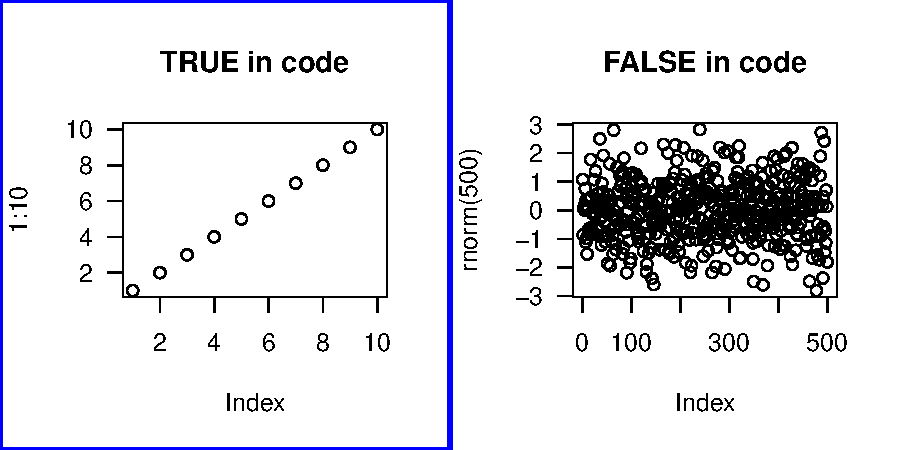
\includegraphics[width=\textwidth]{./fig/cond3-1} 

}



\end{knitrout}
\end{frame}

%------------------------------------------------------------%

\begin{frame}[fragile]{Vectorising: \alert{if}(c) e1 \alert{else} e2 ~~~ vs ~~~ \alert{ifelse}(c, e1, e2)}
\begin{knitrout}
\definecolor{shadecolor}{rgb}{0.961, 0.961, 0.961}\color{fgcolor}\begin{kframe}
\begin{alltt}
\hlstd{v} \hlkwb{<-} \hlkwd{c}\hlstd{(}\hlnum{13}\hlstd{,} \hlnum{14}\hlstd{,} \hlnum{15}\hlstd{,} \hlnum{16}\hlstd{,} \hlnum{17}\hlstd{)}
\hlstd{v}\hlopt{>}\hlnum{14}
\end{alltt}
\begin{verbatim}
## [1] FALSE FALSE  TRUE  TRUE  TRUE
\end{verbatim}
\end{kframe}
\end{knitrout}
\pause
\begin{knitrout}
\definecolor{shadecolor}{rgb}{0.961, 0.961, 0.961}\color{fgcolor}\begin{kframe}
\begin{alltt}
\hlkwd{ifelse}\hlstd{(v}\hlopt{>}\hlnum{14}\hlstd{, v}\hlopt{+}\hlnum{10}\hlstd{,} \hlnum{NA}\hlstd{)} \hlcom{# can handle vector of input}
\end{alltt}
\begin{verbatim}
## [1] NA NA 25 26 27
\end{verbatim}
\end{kframe}
\end{knitrout}
\pause
\begin{knitrout}
\definecolor{shadecolor}{rgb}{0.961, 0.961, 0.961}\color{fgcolor}\begin{kframe}
\begin{alltt}
\hlkwa{if}\hlstd{(v}\hlopt{>}\hlnum{14}\hlstd{) v}\hlopt{+}\hlnum{10} \hlkwa{else} \hlnum{NA}
\end{alltt}


{\ttfamily\noindent\color{warningcolor}{\#\# Warning in if (v > 14) v + 10 else NA: the condition has length > 1 and only the first element will be used}}\begin{verbatim}
## [1] NA
\end{verbatim}
\end{kframe}
\end{knitrout}
\end{frame}

%------------------------------------------------------------%

\begin{frame}[fragile]{Time to practice}
\begin{exercise}{if else - Conditional code execution} %ex
\begin{enumerate}
  \item \rcode{sqrt} returns NaN for the negative values in \rcode{v <- -3:5} and warns about it. With a conditional expression, pass 0 instead of negative values to \rcode{sqrt}.
  \item Construct a statement that checks whether the variable \rcode{input <- 4} is a number smaller than 3. Let it write a useful \rcode{message} to the console (for both cases). Now test it with \rcode{input <- 1.8} and \rcode{input <- -17}.
  \item Now restrict the correct value of input to \emph{positive} numbers <3, i.e. the number must be <3 AND $\geq$ 0.
  \item BONUS 1: What happens if \rcode{input <- "2"} or if \rcode{input <- "b"}?
  \item BONUS 2: Create a character variable that, depending on the result of \rcode{rnorm(1)}, is initiated with probable or unlikely.
  \item BONUS 3: \rcode{replicate} this experiment 1000 times and examine the result with \rcode{table}.
  \item BONUS 4: How could you do this with \rcode{ifelse}?
\end{enumerate}
\end{exercise}
\end{frame}

%------------------------------------------------------------%

\begin{frame}[fragile]{Solution for exercise \arabic{exercisecount}.1: if else}
\begin{knitrout}\footnotesize
\definecolor{shadecolor}{rgb}{0.961, 0.961, 0.961}\color{fgcolor}\begin{kframe}
\begin{alltt}
\hlstd{v} \hlkwb{<-} \hlopt{-}\hlnum{3}\hlopt{:}\hlnum{5}
\hlkwd{sqrt}\hlstd{(v)}
\end{alltt}


{\ttfamily\noindent\color{warningcolor}{\#\# Warning in sqrt(v): NaNs produced}}\begin{verbatim}
## [1]    NaN    NaN    NaN 0.0000 1.0000 1.4142 1.7321 2.0000 2.2361
\end{verbatim}
\end{kframe}
\end{knitrout}
\begin{knitrout}\footnotesize
\definecolor{shadecolor}{rgb}{0.961, 0.961, 0.961}\color{fgcolor}\begin{kframe}
\begin{alltt}
\hlkwd{ifelse}\hlstd{( v} \hlopt{>=} \hlnum{0}\hlstd{,} \hlkwd{sqrt}\hlstd{(v),} \hlnum{0}\hlstd{)}
\end{alltt}


{\ttfamily\noindent\color{warningcolor}{\#\# Warning in sqrt(v): NaNs produced}}\begin{verbatim}
## [1] 0.0000 0.0000 0.0000 0.0000 1.0000 1.4142 1.7321 2.0000 2.2361
\end{verbatim}
\end{kframe}
\end{knitrout}
\begin{knitrout}\footnotesize
\definecolor{shadecolor}{rgb}{0.961, 0.961, 0.961}\color{fgcolor}\begin{kframe}
\begin{alltt}
\hlkwd{sqrt}\hlstd{(}\hlkwd{ifelse}\hlstd{( v} \hlopt{>=} \hlnum{0}\hlstd{, v,} \hlnum{0}\hlstd{))}
\end{alltt}
\begin{verbatim}
## [1] 0.0000 0.0000 0.0000 0.0000 1.0000 1.4142 1.7321 2.0000 2.2361
\end{verbatim}
\end{kframe}
\end{knitrout}
\end{frame}

%------------------------------------------------------------%

\begin{frame}[fragile]{Solution for exercise \arabic{exercisecount}.2: if else}
\begin{knitrout}
\definecolor{shadecolor}{rgb}{0.961, 0.961, 0.961}\color{fgcolor}\begin{kframe}
\begin{alltt}
\hlstd{input} \hlkwb{<-} \hlnum{4}
\hlkwa{if}\hlstd{( input} \hlopt{>=} \hlnum{3} \hlstd{)} \hlkwd{message}\hlstd{(}\hlstr{"Input was wrong.
                         It should be <3"}\hlstd{)} \hlkwa{else}
                 \hlkwd{message}\hlstd{(}\hlstr{"Input OK"}\hlstd{)}
\end{alltt}


{\ttfamily\noindent\itshape\color{messagecolor}{\#\# Input was wrong.\\\#\#\ \ \ \ \ \ \ \ \ \ \ \ \ \ \ \ \ \ \ \ \ \ \ \ \ \ It should be <3}}\begin{alltt}
\hlcom{# run it again after}
\hlstd{input} \hlkwb{<-} \hlnum{1.8}
\hlstd{input} \hlkwb{<-} \hlopt{-}\hlnum{17}
\end{alltt}
\end{kframe}
\end{knitrout}

\end{frame}

%------------------------------------------------------------%

\begin{frame}[fragile]{Solution for exercise \arabic{exercisecount}.3: if else}
\begin{knitrout}
\definecolor{shadecolor}{rgb}{0.961, 0.961, 0.961}\color{fgcolor}\begin{kframe}
\begin{alltt}
\hlcom{# three different solutions:}
\hlkwa{if}\hlstd{( input} \hlopt{>=} \hlnum{3} \hlstd{)} \hlkwd{message}\hlstd{(}\hlstr{"Input is > 3"}\hlstd{)} \hlkwa{else}
\hlkwa{if}\hlstd{( input} \hlopt{<} \hlnum{0} \hlstd{)}  \hlkwd{message}\hlstd{(}\hlstr{"Input is < 0"}\hlstd{)} \hlkwa{else}
                 \hlkwd{message}\hlstd{(}\hlstr{"Input OK"}\hlstd{)}

\hlkwa{if}\hlstd{( input} \hlopt{>=} \hlnum{3} \hlopt{|}  \hlstd{input} \hlopt{<} \hlnum{0}\hlstd{)}
   \hlkwd{message}\hlstd{(}\hlstr{"Input outside 0...3"}\hlstd{)} \hlkwa{else}
   \hlkwd{message}\hlstd{(}\hlstr{"Input OK"}\hlstd{)}

\hlkwa{if}\hlstd{( input} \hlopt{>} \hlnum{0}  \hlopt{&}  \hlstd{input} \hlopt{<=} \hlnum{3} \hlstd{)}   \hlkwd{message}\hlstd{(}\hlstr{"Input OK"}\hlstd{)} \hlkwa{else}
           \hlkwd{message}\hlstd{(}\hlstr{"Input ("}\hlstd{,input,}\hlstr{") outside 0...3"}\hlstd{)}
\end{alltt}
\end{kframe}
\end{knitrout}
\end{frame}

%------------------------------------------------------------%

\begin{frame}[fragile]{Solution for exercise \arabic{exercisecount}.3: if else BONUS}
\begin{knitrout}
\definecolor{shadecolor}{rgb}{0.961, 0.961, 0.961}\color{fgcolor}\begin{kframe}
\begin{alltt}
\hlstd{result} \hlkwb{<-} \hlkwa{if}\hlstd{(}\hlkwd{rnorm}\hlstd{(}\hlnum{1}\hlstd{)}\hlopt{>}\hlnum{2}\hlstd{)} \hlstr{"unlikely"} \hlkwa{else} \hlstr{"probable"}

\hlstd{result} \hlkwb{<-} \hlkwd{replicate}\hlstd{(}\hlkwc{n}\hlstd{=}\hlnum{1000}\hlstd{,} \hlkwc{expr}\hlstd{=}
             \hlkwa{if}\hlstd{(}\hlkwd{rnorm}\hlstd{(}\hlnum{1}\hlstd{)}\hlopt{>}\hlnum{2}\hlstd{)} \hlstr{"unlikely"} \hlkwa{else} \hlstr{"probable"}\hlstd{)}
\hlkwd{table}\hlstd{(result)}

\hlstd{result} \hlkwb{<-} \hlkwd{ifelse}\hlstd{(}\hlkwd{rnorm}\hlstd{(}\hlnum{1000}\hlstd{)}\hlopt{>}\hlnum{2}\hlstd{,} \hlstr{"unlikely"}\hlstd{,} \hlstr{"probable"}\hlstd{)}
\hlkwd{table}\hlstd{(result)}
\end{alltt}
\end{kframe}
\end{knitrout}
\end{frame}

%------------------------------------------------------------%

\begin{frame}[fragile]{Notes on logical values}
\begin{itemize}[<+->]
\item as you might have seen in \rcode{read.table(header=T)}, logical values (TRUE, FALSE) can be abbreviated.
\item If you want to play a mean prank on someone, write\\ \rcode{T <- FALSE; F <- TRUE} in their \href{https://rclickhandbuch.wordpress.com/install-r/rprofile/}{Rprofile} (see \rcode{?Startup}).
\item Logical (boolean) values F and T internally are often converted to integers 0 and 1, thus \rcode{sum(c(T,F,F,T,T,T,F,F,T))} is the number of TRUEs in a vector, \rcode{mean} yields the proportion of TRUEs.
\item \rcode{which(logicalVec)} gives the indices (positions) of TRUE values.
\item \rcode{Vec[logicalVec]} returns only the values of vec corresponding to TRUE in logicalVec (No need to wrap it into \rcode{which}).
\item Logical operators: \rcode{!, \&, |, xor()} (not, and, or, exclusive or)
% \item \rcode{cat(T, letters[c(12,15,22,5)])}
\end{itemize}
\end{frame}

%------------------------------------------------------------%

\begin{frame}[fragile]{Notes on conditional code execution}
\begin{itemize}[<+->]
\item \rcode{\alert{if}(c)\{ex1\}} is valid code, thus R doesn't expect \alert{else} anymore.
\item If you execute code line by line (in a script, for example), \alert{\}} and \alert{else} must be on the same line.
\item Many people consider it good practice to do this in functions as well, but for machine-readability, it is technically fine to write\\
\texttt{\alert{if}(cond)\\
~~\{\\
~~ex1a\\
~~ex1b\\
~~\} \\
\alert{else}\\
~~ex2}
\item \rcode{\alert{if}(logicalValue==TRUE) ...} is usually unnecessary, you can write\\
\onslide<+-> \rcode{\alert{if}(logicalValue) ...}, but sometimes,\\
\onslide<+->  \rcode{\alert{if}(isTRUE(logicalValue)) ...} helps to deal with NAs.
% \item \rcode{cat(T, letters[c(12,15,22,5)])}
\end{itemize}
\end{frame}

%------------------------------------------------------------%

\begin{frame}{Actual usage of if else statements}
See the \rcode{hist} source code: \\
\href{https://github.com/wch/r-source/blob/trunk/src/library/graphics/R/hist.R}{github.com/wch/r-source ~ -> ~ src / library / graphics / R / hist.R}\\[1em]
\pause
\begin{knitrout}
\definecolor{shadecolor}{rgb}{0.961, 0.961, 0.961}\color{fgcolor}\begin{kframe}
\begin{alltt}
\hlstd{mad}
\end{alltt}
\end{kframe}
\end{knitrout}
\pause
Multiple nested conditionals\\
\texttt{\alert{if}(a) b \alert{else} \alert{if}(c) d \alert{else} e}\\
can be avoided with \rcode{switch}.
\end{frame}

\fi % commenting out Conditions section
%------------------------------------------------------------%
%------------------------------------------------------------%
\section{For loops}
%------------------------------------------------------------%
%------------------------------------------------------------%

\begin{frame}[fragile]{For loops}
Execute a block of code several times, with different input values.\\
Syntax: ~ \texttt{\alert{for}(aRunningVariable \alert{in} aSequence)\{ doSomething \}}
\pause
Often, i (for index) is used, thus ~~ \texttt{\alert{for}(i \alert{in} 1:n) \rcode{doThis}(i)}
\pause
\begin{knitrout}
\definecolor{shadecolor}{rgb}{0.961, 0.961, 0.961}\color{fgcolor}\begin{kframe}
\begin{alltt}
\hlkwd{help}\hlstd{(}\hlstr{"for"}\hlstd{)} \hlcom{# needs quotation marks!}
\end{alltt}
\end{kframe}
\end{knitrout}
\pause
\begin{knitrout}
\definecolor{shadecolor}{rgb}{0.961, 0.961, 0.961}\color{fgcolor}\begin{kframe}
\begin{alltt}
\hlkwd{print}\hlstd{(}\hlnum{1}\hlopt{:}\hlnum{2}\hlstd{)}
\hlkwd{print}\hlstd{(}\hlnum{1}\hlopt{:}\hlnum{5}\hlstd{)}
\hlkwd{print}\hlstd{(}\hlnum{1}\hlopt{:}\hlnum{9}\hlstd{)}
\end{alltt}
\end{kframe}
\end{knitrout}
\pause
This is easier and less prone to human errors with:
\pause
\begin{knitrout}
\definecolor{shadecolor}{rgb}{0.961, 0.961, 0.961}\color{fgcolor}\begin{kframe}
\begin{alltt}
\hlkwa{for}\hlstd{(i} \hlkwa{in} \hlkwd{c}\hlstd{(}\hlnum{2}\hlstd{,}\hlnum{5}\hlstd{,}\hlnum{9}\hlstd{) ) \{} \hlkwd{print}\hlstd{(}\hlnum{1}\hlopt{:}\hlstd{i) \}}
\end{alltt}
\begin{verbatim}
## [1] 1 2
## [1] 1 2 3 4 5
## [1] 1 2 3 4 5 6 7 8 9
\end{verbatim}
\end{kframe}
\end{knitrout}
\end{frame}


%------------------------------------------------------------%

\begin{frame}[fragile]{For loops: fill a vector}
\begin{knitrout}
\definecolor{shadecolor}{rgb}{0.961, 0.961, 0.961}\color{fgcolor}\begin{kframe}
\begin{alltt}
\hlstd{v} \hlkwb{<-} \hlkwd{vector}\hlstd{(}\hlkwc{mode}\hlstd{=}\hlstr{"numeric"}\hlstd{,} \hlkwc{length}\hlstd{=}\hlnum{20}\hlstd{)}
\hlstd{v}
\end{alltt}
\begin{verbatim}
##  [1] 0 0 0 0 0 0 0 0 0 0 0 0 0 0 0 0 0 0 0 0
\end{verbatim}
\end{kframe}
\end{knitrout}
\pause \vspace{-1em}
\begin{knitrout}
\definecolor{shadecolor}{rgb}{0.961, 0.961, 0.961}\color{fgcolor}\begin{kframe}
\begin{alltt}
\hlkwa{for}\hlstd{(i} \hlkwa{in} \hlnum{3}\hlopt{:}\hlnum{17}\hlstd{)  \{  v[i]} \hlkwb{<-} \hlstd{(i}\hlopt{+}\hlnum{2}\hlstd{)}\hlopt{^}\hlnum{2}  \hlstd{\}}
\end{alltt}
\end{kframe}
\end{knitrout}
\pause \vspace{-1em}
\begin{knitrout}
\definecolor{shadecolor}{rgb}{0.961, 0.961, 0.961}\color{fgcolor}\begin{kframe}
\begin{alltt}
\hlstd{v} \hlcom{# this code was executed once for each i}
\end{alltt}
\begin{verbatim}
##  [1]   0   0  25  36  49  64  81 100 121
## [10] 144 169 196 225 256 289 324 361   0
## [19]   0   0
\end{verbatim}
\end{kframe}
\end{knitrout}
\pause \vspace{-0.5em}
In R, \rcode{for} loops are slow. Always try to vectorize (the best option, not always possible) or use \rcode{lapply} (saves you the initiation of the empty vector, easier to parallize).
\end{frame}

%------------------------------------------------------------%

\begin{frame}[fragile]{For loops: execute code multiple times I}
\hspace{5em} $y = f(x, n) = \frac{12.5*n}{(n-1)!}*(\frac{n x}{8})^{(n-1)}*e^{-\frac{n x}{8}}$
\begin{knitrout}\footnotesize
\definecolor{shadecolor}{rgb}{0.961, 0.961, 0.961}\color{fgcolor}

{\centering 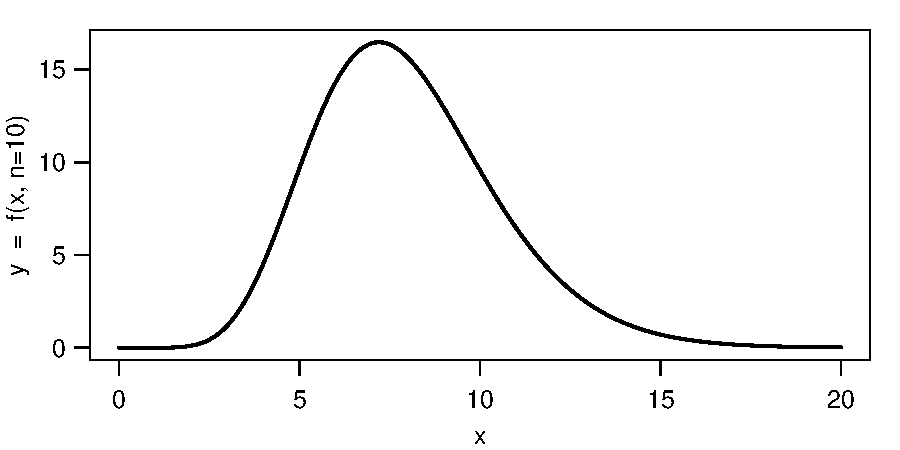
\includegraphics[width=\textwidth]{./fig/for3a-1} 

}



\end{knitrout}

\end{frame}

%------------------------------------------------------------%

\begin{frame}[fragile]{For loops: execute code multiple times II}
\textblockrulecolour{red}
\begin{knitrout}\footnotesize
\definecolor{shadecolor}{rgb}{0.961, 0.961, 0.961}\color{fgcolor}\begin{kframe}
\begin{alltt}
\hlstd{x} \hlkwb{<-} \hlkwd{seq}\hlstd{(}\hlnum{0}\hlstd{,}\hlnum{25}\hlstd{,}\hlnum{0.1}\hlstd{)}
\hlkwd{plot}\hlstd{(x,x,} \hlkwc{type}\hlstd{=}\hlstr{"n"}\hlstd{,} \hlkwc{ylab}\hlstd{=}\hlstr{"y = f(x,n)"}\hlstd{)}
\hlkwd{lines}\hlstd{(x,} \hlnum{12.5}\hlopt{*}\hlnum{5}\hlopt{/}\hlkwd{factorial}\hlstd{(}\hlnum{5}\hlopt{-}\hlnum{1}\hlstd{)}\hlopt{*}\hlstd{(x}\hlopt{/}\hlnum{8}\hlopt{*}\hlnum{5}\hlstd{)}\hlopt{^}\hlstd{(}\hlnum{5}\hlopt{-}\hlnum{1}\hlstd{)}\hlopt{*}\hlkwd{exp}\hlstd{(}\hlopt{-}\hlstd{x}\hlopt{/}\hlnum{8}\hlopt{*}\hlnum{5}\hlstd{),} \hlkwc{col}\hlstd{=}\hlnum{2}\hlstd{)}
\hlkwd{lines}\hlstd{(x,} \hlnum{12.5}\hlopt{*}\hlnum{6}\hlopt{/}\hlkwd{factorial}\hlstd{(}\hlnum{6}\hlopt{-}\hlnum{1}\hlstd{)}\hlopt{*}\hlstd{(x}\hlopt{/}\hlnum{8}\hlopt{*}\hlnum{6}\hlstd{)}\hlopt{^}\hlstd{(}\hlnum{6}\hlopt{-}\hlnum{1}\hlstd{)}\hlopt{*}\hlkwd{exp}\hlstd{(}\hlopt{-}\hlstd{x}\hlopt{/}\hlnum{8}\hlopt{*}\hlnum{6}\hlstd{),} \hlkwc{col}\hlstd{=}\hlnum{2}\hlstd{)}
\end{alltt}
\end{kframe}

{\centering 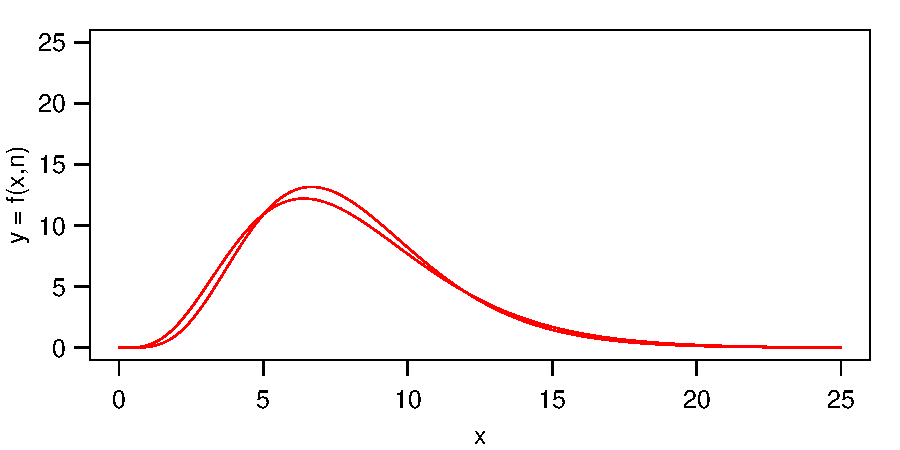
\includegraphics[width=\textwidth]{./fig/for3-1} 

}



\end{knitrout}
\only<2>{
\begin{textblock*}{0.2cm}(2.6cm,2.2cm)
\vspace{0.9cm} ~
\end{textblock*}
%
\begin{textblock*}{0.2cm}(4.6cm,2.2cm)
\vspace{0.9cm} ~
\end{textblock*}
%
\begin{textblock*}{0.2cm}(6.27cm,2.2cm)
\vspace{0.9cm} ~
\end{textblock*}
%
\begin{textblock*}{0.2cm}(6.93cm,2.2cm)
\vspace{0.9cm} ~
\end{textblock*}
%
\begin{textblock*}{0.2cm}(9.25cm,2.2cm)
\vspace{0.9cm} ~
\end{textblock*}
%
}
\end{frame}

%------------------------------------------------------------%

\begin{frame}[fragile]{For loops: execute code multiple times III}
\begin{knitrout}\footnotesize
\definecolor{shadecolor}{rgb}{0.961, 0.961, 0.961}\color{fgcolor}\begin{kframe}
\begin{alltt}
\hlstd{x} \hlkwb{<-} \hlkwd{seq}\hlstd{(}\hlnum{0}\hlstd{,}\hlnum{25}\hlstd{,}\hlnum{0.1}\hlstd{)}
\hlkwd{plot}\hlstd{(x,x,} \hlkwc{type}\hlstd{=}\hlstr{"n"}\hlstd{,} \hlkwc{ylab}\hlstd{=}\hlstr{"y = f(x,n)"}\hlstd{)}
\hlkwa{for} \hlstd{(n} \hlkwa{in} \hlnum{5}\hlopt{:}\hlnum{25}\hlstd{)}
\hlkwd{lines}\hlstd{(x,} \hlnum{12.5}\hlopt{*}\hlstd{n}\hlopt{/}\hlkwd{factorial}\hlstd{(n}\hlopt{-}\hlnum{1}\hlstd{)}\hlopt{*}\hlstd{(x}\hlopt{/}\hlnum{8}\hlopt{*}\hlstd{n)}\hlopt{^}\hlstd{(n}\hlopt{-}\hlnum{1}\hlstd{)}\hlopt{*}\hlkwd{exp}\hlstd{(}\hlopt{-}\hlstd{x}\hlopt{/}\hlnum{8}\hlopt{*}\hlstd{n),} \hlkwc{col}\hlstd{=}\hlnum{2}\hlstd{)}
\end{alltt}
\end{kframe}

{\centering 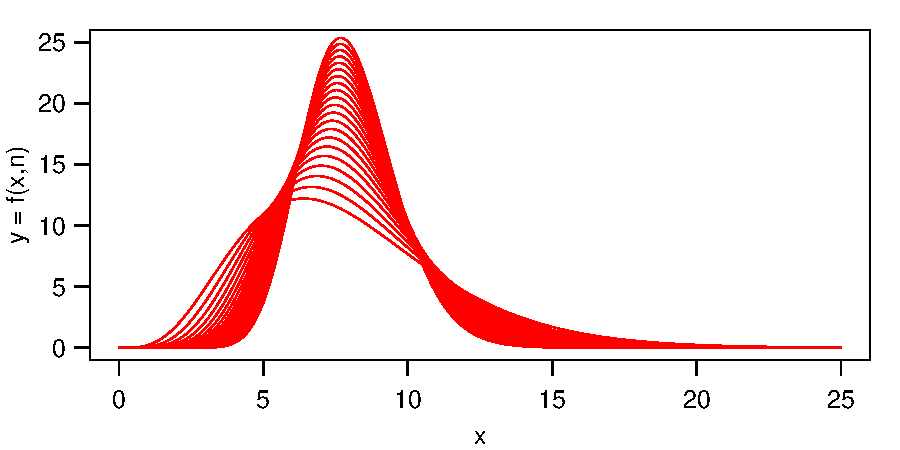
\includegraphics[width=\textwidth]{./fig/for5-1} 

}



\end{knitrout}
\begin{textblock*}{0.2cm}(2.6cm,2.65cm)
\vspace{0.45cm} ~
\end{textblock*}
%
\begin{textblock*}{0.2cm}(4.6cm,2.65cm)
\vspace{0.45cm} ~
\end{textblock*}
%
\begin{textblock*}{0.2cm}(6.27cm,2.65cm)
\vspace{0.45cm} ~
\end{textblock*}
%
\begin{textblock*}{0.2cm}(6.93cm,2.65cm)
\vspace{0.45cm} ~
\end{textblock*}
%
\begin{textblock*}{0.2cm}(9.25cm,2.65cm)
\vspace{0.45cm} ~
\end{textblock*}
%
\end{frame}

%------------------------------------------------------------%

\begin{frame}[fragile]{for loops shouldn't grow a vector}
Bad practice - R needs to recreate the vector each time:
\begin{knitrout}\small
\definecolor{shadecolor}{rgb}{0.961, 0.961, 0.961}\color{fgcolor}\begin{kframe}
\begin{alltt}
\hlstd{output} \hlkwb{<-} \hlnum{NA}
\hlkwa{for}\hlstd{(column} \hlkwa{in} \hlnum{1}\hlopt{:}\hlnum{5}\hlstd{) output[column]} \hlkwb{<-} \hlkwd{median}\hlstd{(iris[ ,column])}
\end{alltt}
\end{kframe}
\end{knitrout}
\pause
This internally does the same thing as:
\begin{knitrout}\small
\definecolor{shadecolor}{rgb}{0.961, 0.961, 0.961}\color{fgcolor}\begin{kframe}
\begin{alltt}
\hlstd{output} \hlkwb{<-} \hlkwd{vector}\hlstd{(}\hlkwc{mode}\hlstd{=}\hlstr{"numeric"}\hlstd{,} \hlkwc{length}\hlstd{=}\hlnum{0}\hlstd{)}
\hlkwa{for}\hlstd{(column} \hlkwa{in} \hlnum{1}\hlopt{:}\hlnum{5}\hlstd{) output} \hlkwb{<-} \hlkwd{c}\hlstd{(output,} \hlkwd{median}\hlstd{(iris[ ,column])  )}
\end{alltt}
\end{kframe}
\end{knitrout}
\pause
Good practice - first tell R how big the output will be, so it can be adequately allocated in memory:
\begin{knitrout}\small
\definecolor{shadecolor}{rgb}{0.961, 0.961, 0.961}\color{fgcolor}\begin{kframe}
\begin{alltt}
\hlstd{output} \hlkwb{<-} \hlkwd{vector}\hlstd{(}\hlkwc{mode}\hlstd{=}\hlstr{"numeric"}\hlstd{,} \hlkwc{length}\hlstd{=}\hlnum{5}\hlstd{)}
\hlkwa{for}\hlstd{(column} \hlkwa{in} \hlnum{1}\hlopt{:}\hlnum{5}\hlstd{) output[column]} \hlkwb{<-} \hlkwd{median}\hlstd{(iris[ ,column])}
\end{alltt}
\end{kframe}
\end{knitrout}
\end{frame}

%------------------------------------------------------------%

\begin{frame}[fragile]{for loops exercise}
\begin{exercise}{for loops in file creation}
\scriptsize
We'll write many datasets to disc (and read them back).
\begin{enumerate}
\item With \rcode{paste0}, print a filename of the structure "mydata\_123.txt" 
      using the name, the number and the file ending as inputs. 
      We'll be changing the number later in a loop.
\item Print a data.frame with two columns, each with 10 random numbers: 
      one column from the normal, one from the exponential distribution
\item With \rcode{write.table}, write such a table to a file in a subfolder (remember \rcode{dir.create}), 
      using the number of rows (e.g. 10) in the filename.\\
\item BONUS: change the arguments so that row numbers and quotation marks are not printed and tabstops are used for column separation.
\item With a \rcode{for}-loop, now write files for different sample sizes, e.g. 10, 20, 50, 100, 500.
\item Using the output of \rcode{dir()}, read all the files into a list of data.frames.
      Remember to first create an empty list of the right length.
\item BONUS: name the list elements according to the filenames. 
\item BONUS: now replace the whole construct with an \rcode{lapply} loop. 
      Celebrate how much nicer your code looks. 
      Check how you can get element names with \rcode{sapply(..., simplify=FALSE)}
\item BONUS: With \rcode{unlink}, delete the files from this exercise. 
      This function is vectorizable, so there's no need to do this in a for loop!
\end{enumerate}
\end{exercise}
\normalsize
\end{frame}

%------------------------------------------------------------%

% \begin{frame}[fragile]{Recap \alert{for} loop}
% \pause
% With \rcode{rexp(n, rate)}, random numbers can be generated from the exponential distribution.\\
% With \rcode{paste0("someText\_", 1)}, character strings and numbers can be concatenated.\\ 
% With \rcode{write.table(x, file)}, data can be written to a file.\\
% Using a \alert{for} loop, write three datasets to separate .txt files with 5, 20 and 100 exponentially distributed random numbers.\\
% BONUS: format the file nicely with the \rcode{write.table()} options. 
% \pause
% <<recapfor, size="small">>=
% for(n in c(5,20,100)) 
%   write.table(rexp(n), file=paste0("random_", n, ".txt"))
% @
% \end{frame}

%------------------------------------------------------------%

\begin{frame}[fragile]{for loops exercise solution}
\begin{knitrout}\footnotesize
\definecolor{shadecolor}{rgb}{0.961, 0.961, 0.961}\color{fgcolor}\begin{kframe}
\begin{alltt}
\hlkwd{dir.create}\hlstd{(}\hlstr{"loopexercise"}\hlstd{)}
\hlkwa{for}\hlstd{(n} \hlkwa{in} \hlkwd{c}\hlstd{(}\hlnum{10}\hlstd{,}\hlnum{20}\hlstd{,}\hlnum{50}\hlstd{,}\hlnum{100}\hlstd{,}\hlnum{500}\hlstd{))}
    \hlkwd{write.table}\hlstd{(}\hlkwc{x}\hlstd{=}\hlkwd{data.frame}\hlstd{(}\hlkwc{norm}\hlstd{=}\hlkwd{rnorm}\hlstd{(n),} \hlkwc{exp}\hlstd{=}\hlkwd{rexp}\hlstd{(n)),}
                \hlkwc{file}\hlstd{=}\hlkwd{paste0}\hlstd{(}\hlstr{"loopexercise/randomdata_"}\hlstd{, n,} \hlstr{".txt"}\hlstd{),}
                \hlkwc{quote}\hlstd{=F,} \hlkwc{row.names}\hlstd{=F,} \hlkwc{sep}\hlstd{=}\hlstr{"\textbackslash{}t"}\hlstd{)}

\hlstd{fnames} \hlkwb{<-} \hlkwd{dir}\hlstd{(}\hlstr{"loopexercise"}\hlstd{,} \hlkwc{full}\hlstd{=}\hlnum{TRUE}\hlstd{)}
\hlstd{fcontents} \hlkwb{<-} \hlkwd{vector}\hlstd{(}\hlstr{"list"}\hlstd{,} \hlkwc{length}\hlstd{=}\hlkwd{length}\hlstd{(fnames))}
\hlkwa{for}\hlstd{(fnum} \hlkwa{in} \hlkwd{seq_along}\hlstd{(fnames))}
   \hlstd{fcontents[[fnum]]} \hlkwb{<-} \hlkwd{read.table}\hlstd{(fnames[fnum],} \hlkwc{header}\hlstd{=}\hlnum{TRUE}\hlstd{)}

\hlstd{flist} \hlkwb{<-} \hlkwd{sapply}\hlstd{(}\hlkwd{dir}\hlstd{(}\hlstr{"loopexercise"}\hlstd{,} \hlkwc{full}\hlstd{=}\hlnum{TRUE}\hlstd{), read.table,} \hlkwc{header}\hlstd{=}\hlnum{TRUE}\hlstd{,}
                \hlkwc{simplify}\hlstd{=}\hlnum{FALSE}\hlstd{)}

\hlkwd{unlink}\hlstd{(}\hlkwd{paste0}\hlstd{(}\hlstr{"loopexercise/randomdata_"}\hlstd{,} \hlkwd{c}\hlstd{(}\hlnum{10}\hlstd{,}\hlnum{20}\hlstd{,}\hlnum{50}\hlstd{,}\hlnum{100}\hlstd{,}\hlnum{500}\hlstd{),} \hlstr{".txt"}\hlstd{))}
\end{alltt}
\end{kframe}
\end{knitrout}
\end{frame}

%------------------------------------------------------------%

\begin{frame}[fragile]{\rcode{seq\_along(n)} is safer than \rcode{1:n} in \alert{for} loops}
\pause
\vspace{-0.5em}
\begin{knitrout}\scriptsize
\definecolor{shadecolor}{rgb}{0.961, 0.961, 0.961}\color{fgcolor}\begin{kframe}
\begin{alltt}
\hlstd{do_something} \hlkwb{<-} \hlkwa{function}\hlstd{(}\hlkwc{x}\hlstd{)} \hlkwa{if}\hlstd{(x}\hlopt{<}\hlnum{1}\hlstd{)} \hlkwd{stop}\hlstd{(}\hlstr{"x must be >=1, not:"}\hlstd{, x)} \hlkwa{else} \hlstd{x}
\hlstd{something} \hlkwb{<-} \hlnum{1}\hlopt{:}\hlnum{6}
\end{alltt}
\end{kframe}
\end{knitrout}
\pause
You'll often see the dangerous code \rcode{\alert{for}(i in 1:n)}: \vspace{-0.7em}
\begin{knitrout}\footnotesize
\definecolor{shadecolor}{rgb}{0.961, 0.961, 0.961}\color{fgcolor}\begin{kframe}
\begin{alltt}
\hlkwa{for}\hlstd{(i} \hlkwa{in} \hlnum{1}\hlopt{:}\hlkwd{length}\hlstd{(something))} \hlkwd{do_something}\hlstd{(i)} \hlcom{# works with current sth}
\end{alltt}
\end{kframe}
\end{knitrout}
\pause
Imagine this:\vspace{-0.5em}
\begin{knitrout}\footnotesize
\definecolor{shadecolor}{rgb}{0.961, 0.961, 0.961}\color{fgcolor}\begin{kframe}
\begin{alltt}
\hlstd{something} \hlkwb{<-} \hlkwd{which}\hlstd{(letters}\hlopt{==}\hlstr{"4"}\hlstd{)}
\hlkwa{for}\hlstd{(i} \hlkwa{in} \hlnum{1}\hlopt{:}\hlkwd{length}\hlstd{(something))} \hlkwd{do_something}\hlstd{(i)} \hlcom{# fails! (same code!)}
\end{alltt}


{\ttfamily\noindent\bfseries\color{errorcolor}{\#\# Error in do\_something(i): x must be >=1, not:0}}\end{kframe}
\end{knitrout}
\pause
Safer to use is:\vspace{-0.7em}
\begin{knitrout}
\definecolor{shadecolor}{rgb}{0.961, 0.961, 0.961}\color{fgcolor}\begin{kframe}
\begin{alltt}
\hlkwa{for}\hlstd{(i} \hlkwa{in} \hlkwd{seq_along}\hlstd{(something))} \hlkwd{do_something}\hlstd{(i)}
\end{alltt}
\end{kframe}
\end{knitrout}
\pause
Because:\vspace{-0.5em}
\begin{knitrout}\scriptsize
\definecolor{shadecolor}{rgb}{0.961, 0.961, 0.961}\color{fgcolor}\begin{kframe}
\begin{alltt}
\hlnum{1}\hlopt{:}\hlkwd{length}\hlstd{(something)     ;}   \hlkwd{seq_along}\hlstd{(something)}
\end{alltt}
\begin{verbatim}
## [1] 1 0
## integer(0)
\end{verbatim}
\end{kframe}
\end{knitrout}
\end{frame}

%------------------------------------------------------------%

\begin{frame}[fragile]{stocks data from \href{http://finance.yahoo.com}{finance.yahoo.com}}
\begin{knitrout}\scriptsize
\definecolor{shadecolor}{rgb}{0.961, 0.961, 0.961}\color{fgcolor}\begin{kframe}
\begin{alltt}
\hlcom{# Download current datasets:}
\hlkwa{if}\hlstd{(}\hlopt{!}\hlkwd{requireNamespace}\hlstd{(}\hlstr{"quantmod"}\hlstd{))} \hlkwd{install.packages}\hlstd{(}\hlstr{"quantmod"}\hlstd{)}
\hlkwa{if}\hlstd{(}\hlopt{!}\hlkwd{requireNamespace}\hlstd{(}\hlstr{"pbapply"}\hlstd{))}  \hlkwd{install.packages}\hlstd{(}\hlstr{"pbapply"}\hlstd{)}
\hlstd{dummy} \hlkwb{<-} \hlstd{pbapply}\hlopt{::}\hlkwd{pblapply}\hlstd{(}\hlkwd{c}\hlstd{(}\hlstr{"F"}\hlstd{,}\hlstr{"VLKAF"}\hlstd{,} \hlstr{"AMZN"}\hlstd{,}\hlstr{"AAPL"}\hlstd{,}\hlstr{"GOOG"}\hlstd{,}\hlstr{"MSFT"}\hlstd{),}
   \hlkwa{function}\hlstd{(}\hlkwc{x}\hlstd{) zoo}\hlopt{::}\hlkwd{write.zoo}\hlstd{(}\hlkwc{x}\hlstd{=quantmod}\hlopt{::}\hlkwd{getSymbols}\hlstd{(x,} \hlkwc{auto.assign}\hlstd{=}\hlnum{FALSE}\hlstd{)[,}\hlnum{6}\hlstd{],}
                           \hlkwc{file}\hlstd{=}\hlkwd{paste0}\hlstd{(}\hlstr{"data/finance/"}\hlstd{,x,}\hlstr{".txt"}\hlstd{),} \hlkwc{col.names}\hlstd{=T))}

\hlcom{# read single files to R and merge into one file:}
\hlstd{stocks} \hlkwb{<-} \hlkwd{lapply}\hlstd{(}\hlkwd{dir}\hlstd{(}\hlstr{"data/finance"}\hlstd{,} \hlkwc{full}\hlstd{=}\hlnum{TRUE}\hlstd{),}
                  \hlstd{read.table,} \hlkwc{as.is}\hlstd{=}\hlnum{TRUE}\hlstd{,} \hlkwc{header}\hlstd{=}\hlnum{TRUE}\hlstd{)}
\hlstd{stocks} \hlkwb{<-} \hlkwd{Reduce}\hlstd{(}\hlkwa{function}\hlstd{(}\hlkwc{...}\hlstd{)} \hlkwd{merge}\hlstd{(...,} \hlkwc{all}\hlstd{=T), stocks)}

\hlcom{# Get nicer column names:}
\hlstd{names} \hlkwb{<-} \hlkwd{sapply}\hlstd{(}\hlkwd{strsplit}\hlstd{(}\hlkwd{colnames}\hlstd{(stocks),} \hlstr{"."}\hlstd{,} \hlkwc{fix}\hlstd{=}\hlnum{TRUE}\hlstd{),}\hlstr{"["}\hlstd{,} \hlnum{1}\hlstd{)}
\hlkwd{colnames}\hlstd{(stocks)} \hlkwb{<-} \hlkwd{c}\hlstd{(}\hlkwc{Index}\hlstd{=}\hlstr{"Date"}\hlstd{,} \hlkwc{F}\hlstd{=}\hlstr{"FORD"}\hlstd{,} \hlkwc{VLKAF}\hlstd{=}\hlstr{"VOLKSWAGEN"}\hlstd{,}
         \hlkwc{AMZN}\hlstd{=}\hlstr{"AMAZON"}\hlstd{,} \hlkwc{AAPL}\hlstd{=}\hlstr{"APPLE"}\hlstd{,} \hlkwc{GOOG}\hlstd{=}\hlstr{"GOOGLE"}\hlstd{,} \hlkwc{MSFT}\hlstd{=}\hlstr{"MICROSOFT"}\hlstd{)[names]}

\hlcom{# Save to disc:}
\hlkwd{write.table}\hlstd{(stocks,} \hlkwc{file}\hlstd{=}\hlstr{"data/stocks.txt"}\hlstd{,} \hlkwc{row.names}\hlstd{=F,} \hlkwc{quote}\hlstd{=F)}
\end{alltt}
\end{kframe}
\end{knitrout}
\end{frame}

%------------------------------------------------------------%

\begin{frame}[fragile]{For loops: multipanel graphics: the task}
\begin{exercise}{for loop}
\begin{enumerate}
\item Read \datalinkText{stocks.txt}, so that there are no factors in the data.frame
\item Change the first column type from \texttt{char} to \texttt{date} with \rcode{?as.Date}
\item What do you get with \rcode{plot(stocks[ ,1:2])}? Make it a line graph.
\item With \rcode{par(mfrow...}, set up a two by three panel plot
\item With a for loop, fill those with each stock time series
\item BONUS 1: Make good annotations, including a main title (par oma, \rcode{mtext} with the outer argument)
\item BONUS 2: Make the plot margins smaller (par mar), turn y axis labels upright (las) and move the axis labels closer to the plots (mgp).
\item BONUS 3: Understand and comment each line of the data preparation. %Get your own files or use mine: \footnotesize{\datalinkBlob{finance/AAPL.txt}, \datalinkBlob{finance/AMZN.txt}, \datalinkBlob{finance/F.txt}, \datalinkBlob{finance/GOOG.txt}, \datalinkBlob{finance/VLKAY.txt}, \datalinkBlob{finance/YHOO.txt}}
\end{enumerate}
\end{exercise}
\end{frame}

%------------------------------------------------------------%

\begin{frame}[fragile]{For loops: multipanel graphics: the solution}
\vspace{-1em}
\begin{knitrout}\footnotesize
\definecolor{shadecolor}{rgb}{0.961, 0.961, 0.961}\color{fgcolor}\begin{kframe}
\begin{alltt}
\hlstd{stocks} \hlkwb{<-} \hlkwd{read.table}\hlstd{(}\hlstr{"data/stocks.txt"}\hlstd{,} \hlkwc{header}\hlstd{=T,} \hlkwc{as.is}\hlstd{=T)}
\hlstd{stocks}\hlopt{$}\hlstd{Date} \hlkwb{<-} \hlkwd{as.Date}\hlstd{(stocks}\hlopt{$}\hlstd{Date)}
\hlkwd{par}\hlstd{(}\hlkwc{mfrow}\hlstd{=}\hlkwd{c}\hlstd{(}\hlnum{2}\hlstd{,}\hlnum{3}\hlstd{),} \hlkwc{mar}\hlstd{=}\hlkwd{c}\hlstd{(}\hlnum{2}\hlstd{,}\hlnum{4}\hlstd{,}\hlnum{1}\hlstd{,}\hlnum{1}\hlstd{),} \hlkwc{mgp}\hlstd{=}\hlkwd{c}\hlstd{(}\hlnum{2.5}\hlstd{,}\hlnum{0.7}\hlstd{,}\hlnum{0}\hlstd{),}\hlkwc{oma}\hlstd{=}\hlkwd{c}\hlstd{(}\hlnum{0}\hlstd{,}\hlnum{0}\hlstd{,}\hlnum{2}\hlstd{,}\hlnum{0}\hlstd{),}\hlkwc{las}\hlstd{=}\hlnum{1}\hlstd{)}
\hlkwa{for}\hlstd{(i} \hlkwa{in} \hlnum{2}\hlopt{:}\hlnum{7}\hlstd{)} \hlkwd{plot}\hlstd{(stocks[ ,}\hlkwd{c}\hlstd{(}\hlnum{1}\hlstd{,i)],} \hlkwc{type}\hlstd{=}\hlstr{"l"}\hlstd{)}
\hlkwd{mtext}\hlstd{(}\hlstr{"stocks this decade"}\hlstd{,} \hlkwc{line}\hlstd{=}\hlnum{0}\hlstd{,} \hlkwc{outer}\hlstd{=}\hlnum{TRUE}\hlstd{)}
\end{alltt}
\end{kframe}

{\centering 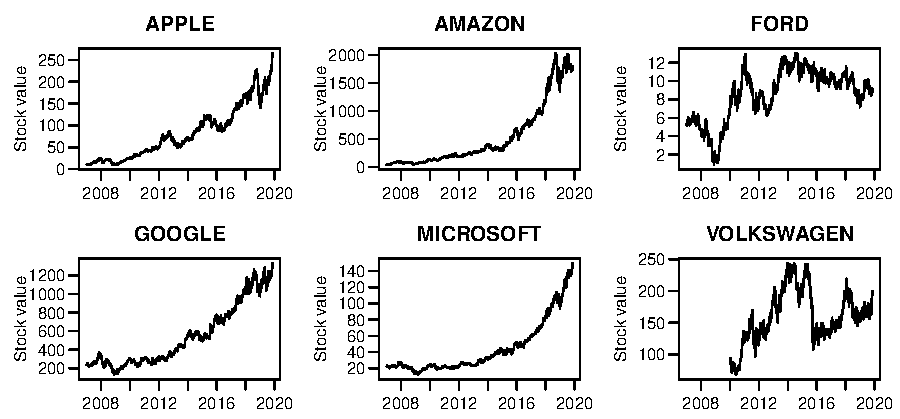
\includegraphics[width=\textwidth]{./fig/forpanel-1} 

}



\end{knitrout}
\end{frame}

%------------------------------------------------------------%

\begin{frame}[fragile]{For loops: multipanel graphics: beautifuller}
\vspace{-1em}
\begin{knitrout}\scriptsize
\definecolor{shadecolor}{rgb}{0.961, 0.961, 0.961}\color{fgcolor}\begin{kframe}
\begin{alltt}
\hlkwd{par}\hlstd{(}\hlkwc{mfrow}\hlstd{=}\hlkwd{c}\hlstd{(}\hlnum{1}\hlstd{,}\hlnum{2}\hlstd{),} \hlkwc{mar}\hlstd{=}\hlkwd{c}\hlstd{(}\hlnum{4}\hlstd{,}\hlnum{4}\hlstd{,}\hlnum{2}\hlstd{,}\hlnum{0.1}\hlstd{),} \hlkwc{mgp}\hlstd{=}\hlkwd{c}\hlstd{(}\hlnum{2.5}\hlstd{,}\hlnum{0.7}\hlstd{,}\hlnum{0}\hlstd{),} \hlkwc{cex}\hlstd{=}\hlnum{0.7}\hlstd{,} \hlkwc{las}\hlstd{=}\hlnum{1}\hlstd{)}
\hlkwa{for}\hlstd{(i} \hlkwa{in} \hlnum{2}\hlopt{:}\hlnum{3}\hlstd{)}
 \hlstd{\{}
 \hlkwd{plot}\hlstd{(stocks[ stocks}\hlopt{$}\hlstd{Date}\hlopt{>}\hlkwd{as.Date}\hlstd{(}\hlstr{"2016-04-01"}\hlstd{) ,} \hlkwd{c}\hlstd{(}\hlnum{1}\hlstd{,i) ],}
      \hlkwc{main}\hlstd{=}\hlkwd{colnames}\hlstd{(stocks)[i],} \hlkwc{xaxt}\hlstd{=}\hlstr{"n"}\hlstd{,} \hlkwc{type}\hlstd{=}\hlstr{"l"}\hlstd{,} \hlkwc{xlab}\hlstd{=}\hlstr{" "}\hlstd{,}
      \hlkwc{ylab}\hlstd{=}\hlkwa{if}\hlstd{(i}\hlopt{==}\hlnum{2}\hlstd{)} \hlstr{"Adjusted daily share price  [USD]"} \hlkwa{else} \hlstr{""}\hlstd{)}
 \hlstd{berryFunctions}\hlopt{::}\hlkwd{monthAxis}\hlstd{(}\hlnum{1}\hlstd{)}
 \hlstd{\}}
\end{alltt}
\end{kframe}

{\centering 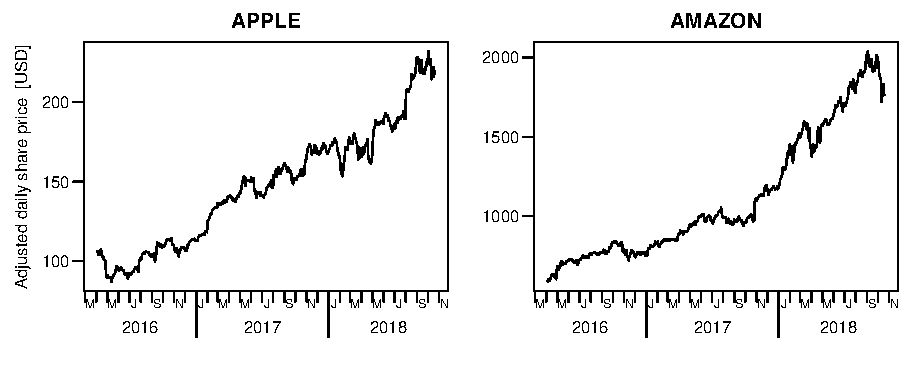
\includegraphics[width=\textwidth]{./fig/forpanel2-1} 

}



\end{knitrout}
\end{frame}

\iffalse % commenting out lapply section
%------------------------------------------------------------%
%------------------------------------------------------------%
\section{lapply}
%------------------------------------------------------------%
%------------------------------------------------------------%

\begin{frame}[fragile]{for -> lapply I: basics}
\vspace{-1em}
\begin{knitrout}
\definecolor{shadecolor}{rgb}{0.961, 0.961, 0.961}\color{fgcolor}\begin{kframe}
\begin{alltt}
\hlstd{files} \hlkwb{<-} \hlkwd{dir}\hlstd{(}\hlstr{"../rawdata"}\hlstd{,} \hlkwc{pattern}\hlstd{=}\hlstr{"*.csv"}\hlstd{,} \hlkwc{full}\hlstd{=}\hlnum{TRUE}\hlstd{)}

\hlcom{#}
\end{alltt}
\end{kframe}
\end{knitrout}
\pause \vspace{-2.7em}
\begin{knitrout}
\definecolor{shadecolor}{rgb}{0.961, 0.961, 0.961}\color{fgcolor}\begin{kframe}
\begin{alltt}
\hlcom{# bad and slow way:}
\hlstd{ldfs} \hlkwb{<-} \hlkwd{list}\hlstd{()} \hlcom{# initiate empty list}
\hlkwa{for}\hlstd{(i} \hlkwa{in} \hlnum{1}\hlopt{:}\hlkwd{length}\hlstd{(files))}
   \hlstd{ldfs[[i]]} \hlkwb{<-} \hlkwd{read.csv}\hlstd{(files[i],} \hlkwc{as.is}\hlstd{=}\hlnum{TRUE}\hlstd{)}

\hlcom{#}
\end{alltt}
\end{kframe}
\end{knitrout}
\pause \vspace{-2.7em}
\begin{knitrout}
\definecolor{shadecolor}{rgb}{0.961, 0.961, 0.961}\color{fgcolor}\begin{kframe}
\begin{alltt}
\hlcom{# much better way: apply function to each file}
\hlstd{ldfs} \hlkwb{<-} \hlkwd{lapply}\hlstd{(}\hlkwc{X}\hlstd{=files,} \hlkwc{FUN}\hlstd{=read.csv,} \hlkwc{as.is}\hlstd{=}\hlnum{TRUE}\hlstd{)}

\hlcom{#}
\end{alltt}
\end{kframe}
\end{knitrout}
\pause \vspace{-2.7em}
\begin{knitrout}
\definecolor{shadecolor}{rgb}{0.961, 0.961, 0.961}\color{fgcolor}\begin{kframe}
\begin{alltt}
\hlcom{# single data.frame if all files have n columns:}
\hlstd{df} \hlkwb{<-} \hlkwd{do.call}\hlstd{(rbind, ldfs)}

\hlcom{#}
\end{alltt}
\end{kframe}
\end{knitrout}
\pause \vspace{-2.7em}
\begin{knitrout}
\definecolor{shadecolor}{rgb}{0.961, 0.961, 0.961}\color{fgcolor}\begin{kframe}
\begin{alltt}
\hlcom{# PS: much faster in this example could be}
\hlkwd{library}\hlstd{(}\hlstr{"data.table"}\hlstd{)} \hlcom{# fread + rbindlist}
\hlstd{ldfs} \hlkwb{<-} \hlkwd{lapply}\hlstd{(}\hlkwc{X}\hlstd{=files,} \hlkwc{FUN}\hlstd{=fread,} \hlkwc{sep}\hlstd{=}\hlstr{","}\hlstd{)}
\hlstd{df} \hlkwb{<-} \hlkwd{rbindlist}\hlstd{(ldfs)}
\end{alltt}
\end{kframe}
\end{knitrout}
\end{frame}

%------------------------------------------------------------%

\begin{frame}[fragile]{for -> lapply II: progress bar, names, indexing etc}
\vspace{-0.6em}
\begin{knitrout}
\definecolor{shadecolor}{rgb}{0.961, 0.961, 0.961}\color{fgcolor}\begin{kframe}
\begin{alltt}
\hlstd{ldfs} \hlkwb{<-}   \hlkwd{lapply}\hlstd{(}\hlkwc{X}\hlstd{=files,} \hlkwc{FUN}\hlstd{=read.csv,} \hlkwc{as.is}\hlstd{=}\hlnum{TRUE}\hlstd{)}

\hlcom{#}
\end{alltt}
\end{kframe}
\end{knitrout}
\pause \vspace{-3.48em}
\begin{knitrout}
\definecolor{shadecolor}{rgb}{0.961, 0.961, 0.961}\color{fgcolor}\begin{kframe}
\begin{alltt}
\hlcom{# progress bar with remaining time}
\hlkwd{library}\hlstd{(}\hlstr{"pbapply"}\hlstd{)}
\hlstd{ldfs} \hlkwb{<-} \hlkwd{pblapply}\hlstd{(}\hlkwc{X}\hlstd{=files,} \hlkwc{FUN}\hlstd{=read.csv,} \hlkwc{as.is}\hlstd{=}\hlnum{TRUE}\hlstd{)}

\hlcom{#}
\end{alltt}
\end{kframe}
\end{knitrout}
\pause \vspace{-3.48em}
\begin{knitrout}
\definecolor{shadecolor}{rgb}{0.961, 0.961, 0.961}\color{fgcolor}\begin{kframe}
\begin{alltt}
\hlcom{# nice additional stuff:}
\hlkwd{names}\hlstd{(ldfs)} \hlkwb{<-} \hlstd{files}
\hlkwd{str}\hlstd{(ldfs,} \hlkwc{max.level}\hlstd{=}\hlnum{1}\hlstd{)}
\hlstd{ldfs[[}\hlnum{2}\hlstd{]]} \hlcom{# second list element}

\hlcom{#}
\end{alltt}
\end{kframe}
\end{knitrout}
\pause \vspace{-3.58em}
\begin{knitrout}
\definecolor{shadecolor}{rgb}{0.961, 0.961, 0.961}\color{fgcolor}\begin{kframe}
\begin{alltt}
\hlcom{# get third column / fifth row from each df:}
\hlkwd{sapply}\hlstd{(ldfs,} \hlstr{"["}\hlstd{,  ,} \hlkwc{j}\hlstd{=}\hlnum{3}\hlstd{)}
\hlkwd{sapply}\hlstd{(ldfs,} \hlstr{"["}\hlstd{,} \hlnum{5}\hlstd{,    )}
\end{alltt}
\end{kframe}
\end{knitrout}
\end{frame}

\fi % commenting out lapply section
%------------------------------------------------------------%
%------------------------------------------------------------%
\section{Functions}
%------------------------------------------------------------%
%------------------------------------------------------------%

\begin{frame}[fragile]{Functions I}
\label{functions1}
\href{http://r4ds.had.co.nz/functions.html}{http://r4ds.had.co.nz/functions.html}\\
\pause
\rcode{?"function"}\\
\pause  Syntax:\\
\rcode{Functionobjectname <- \alert{function}(argument1, argument2, ...) \\
~~~~~~~~~~~~~~~~~~~~~~~~~~~~~~\{"DoSomething"\}}\\
\pause
\begin{knitrout}
\definecolor{shadecolor}{rgb}{0.961, 0.961, 0.961}\color{fgcolor}\begin{kframe}
\begin{alltt}
\hlstd{myfunct} \hlkwb{<-} \hlkwa{function}\hlstd{(}\hlkwc{grappig}\hlstd{)}
       \hlstd{\{}\hlkwd{plot}\hlstd{(grappig,} \hlkwc{type}\hlstd{=}\hlstr{"l"}\hlstd{);} \hlkwd{return}\hlstd{(grappig}\hlopt{*}\hlnum{7}\hlstd{)  \}}
\end{alltt}
\end{kframe}
\end{knitrout}
\pause
After \rcode{return()}ing, the execution of the function is terminated, so it should only be positioned at the end. It can also be left away, the last instruction ("expression") will then be returned.
\end{frame}

%------------------------------------------------------------%

\begin{frame}[fragile]{Functions II}
\begin{knitrout}
\definecolor{shadecolor}{rgb}{0.961, 0.961, 0.961}\color{fgcolor}\begin{kframe}
\begin{alltt}
\hlkwd{myfunct}\hlstd{(}   \hlkwd{c}\hlstd{(}\hlnum{5}\hlstd{,}\hlnum{11}\hlstd{,}\hlnum{3}\hlstd{,}\hlnum{7}\hlstd{)  )}
\end{alltt}
\begin{verbatim}
## [1] 35 77 21 49
\end{verbatim}
\end{kframe}

{\centering 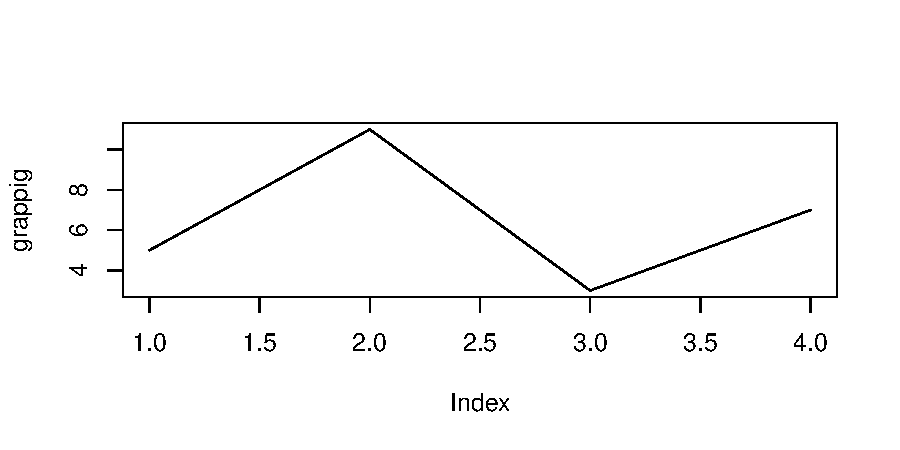
\includegraphics[width=\textwidth]{./fig/funct3-1} 

}



\end{knitrout}
\end{frame}

%------------------------------------------------------------%

\begin{frame}[fragile]{Functions with more arguments}
\begin{knitrout}\small
\definecolor{shadecolor}{rgb}{0.961, 0.961, 0.961}\color{fgcolor}\begin{kframe}
\begin{alltt}
\hlstd{myfunct} \hlkwb{<-} \hlkwa{function}\hlstd{(}\hlkwc{x}\hlstd{,} \hlkwc{type}\hlstd{=}\hlstr{"o"}\hlstd{,} \hlkwc{...}\hlstd{)} \hlkwd{plot}\hlstd{(x,} \hlkwc{type}\hlstd{=type, ...)}
\hlcom{# type="o" is now the default, thus used unless specified}
\hlcom{# The ellipsis (...) passes arguments to other functions}
\hlkwd{myfunct}\hlstd{(}  \hlkwd{c}\hlstd{(}\hlnum{5}\hlstd{,}\hlnum{11}\hlstd{,}\hlnum{3}\hlstd{,}\hlnum{7}\hlstd{) ,} \hlkwc{col}\hlstd{=}\hlstr{"red"}\hlstd{,} \hlkwc{las}\hlstd{=}\hlnum{1}\hlstd{)}
\end{alltt}
\end{kframe}

{\centering 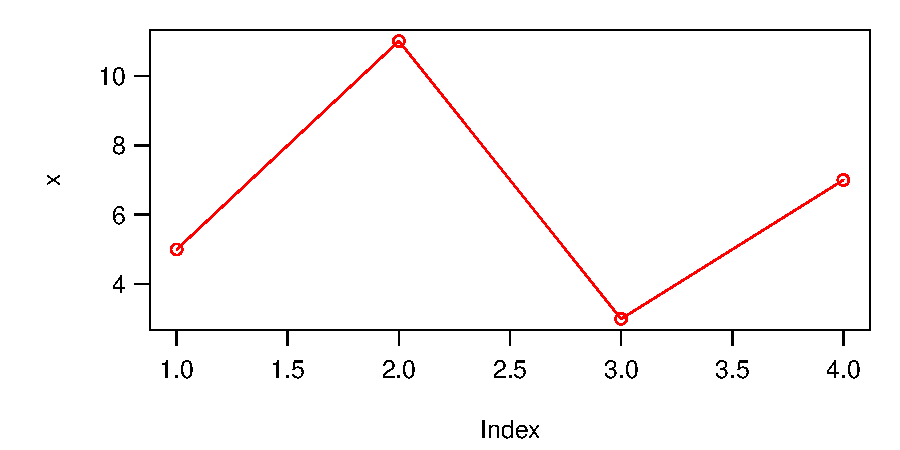
\includegraphics[width=\textwidth]{./fig/funct4-1} 

}



\end{knitrout}
\vspace{-2em}
\end{frame}

%------------------------------------------------------------%

\begin{frame}[fragile]{Functions: example I}
If you needed to find the zeros of quadratic functions very often, you could use
\begin{knitrout}
\definecolor{shadecolor}{rgb}{0.961, 0.961, 0.961}\color{fgcolor}\begin{kframe}
\begin{alltt}
\hlstd{pq} \hlkwb{<-} \hlkwa{function}\hlstd{(}\hlkwc{p}\hlstd{,}\hlkwc{q}\hlstd{)} \hlcom{# y = x^2 + px + q}
              \hlstd{\{}
              \hlstd{w} \hlkwb{<-} \hlkwd{sqrt}\hlstd{( p}\hlopt{^}\hlnum{2} \hlopt{/} \hlnum{4} \hlopt{-} \hlstd{q )}
              \hlkwd{c}\hlstd{(}\hlopt{-}\hlstd{p}\hlopt{/}\hlnum{2}\hlopt{-}\hlstd{w,} \hlopt{-}\hlstd{p}\hlopt{/}\hlnum{2}\hlopt{+}\hlstd{w)}
              \hlstd{\}} \hlcom{# End of function}

\hlkwd{pq}\hlstd{(}\hlnum{3}\hlstd{,} \hlopt{-}\hlnum{12}\hlstd{)}
\end{alltt}
\begin{verbatim}
## [1] -5.274917  2.274917
\end{verbatim}
\end{kframe}
\end{knitrout}
\end{frame}

%------------------------------------------------------------%

\begin{frame}[fragile]{Functions: example II}
\begin{knitrout}
\definecolor{shadecolor}{rgb}{0.961, 0.961, 0.961}\color{fgcolor}\begin{kframe}
\begin{alltt}
\hlstd{x} \hlkwb{<-} \hlkwd{seq}\hlstd{(}\hlopt{-}\hlnum{10}\hlstd{,} \hlnum{10}\hlstd{,} \hlkwc{len}\hlstd{=}\hlnum{100}\hlstd{)}
\hlkwd{plot}\hlstd{(x,  x}\hlopt{^}\hlnum{2} \hlopt{+}\hlnum{3}\hlopt{*}\hlstd{x} \hlopt{-}\hlnum{12}\hlstd{,} \hlkwc{type}\hlstd{=}\hlstr{"l"}\hlstd{,} \hlkwc{col}\hlstd{=}\hlnum{2}\hlstd{)}
\hlkwd{abline}\hlstd{(}\hlkwc{h}\hlstd{=}\hlnum{0}\hlstd{,} \hlkwc{v}\hlstd{=}\hlnum{0}\hlstd{)}
\end{alltt}
\end{kframe}

{\centering 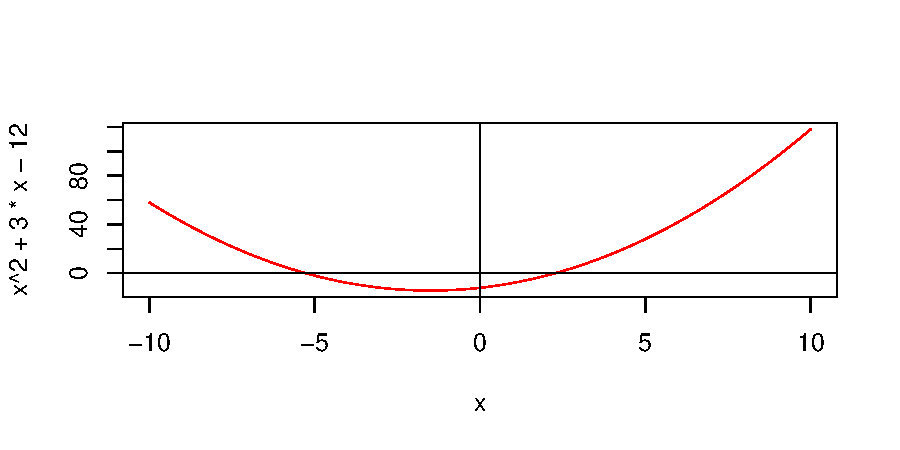
\includegraphics[width=\textwidth]{./fig/pqfunplot-1} 

}



\end{knitrout}
\end{frame}

%------------------------------------------------------------%

\begin{frame}[fragile]{Exercise: add circles with given radius}
\begin{knitrout}
\definecolor{shadecolor}{rgb}{0.961, 0.961, 0.961}\color{fgcolor}\begin{kframe}
\begin{alltt}
\hlkwd{plot}\hlstd{(}\hlnum{1}\hlopt{:}\hlnum{10}\hlstd{,} \hlkwc{asp}\hlstd{=}\hlnum{1}\hlstd{)} \hlcom{# aspect ratio y/x of graph range}
\hlkwd{grid}\hlstd{(}\hlkwc{col}\hlstd{=}\hlnum{1}\hlstd{)} \hlcom{# the next part sould go into a function:}
\hlstd{x} \hlkwb{<-} \hlnum{8} \hlstd{;  y} \hlkwb{<-} \hlnum{6} \hlstd{;  r} \hlkwb{<-}\hlnum{2}
\hlstd{p} \hlkwb{<-} \hlkwd{seq}\hlstd{(}\hlnum{0}\hlstd{,} \hlnum{2}\hlopt{*}\hlstd{pi,} \hlkwc{len}\hlstd{=}\hlnum{50}\hlstd{)}
\hlstd{cx} \hlkwb{<-} \hlstd{x}\hlopt{+}\hlstd{r}\hlopt{*}\hlkwd{cos}\hlstd{(p) ;  cy} \hlkwb{<-} \hlstd{y}\hlopt{+}\hlstd{r}\hlopt{*}\hlkwd{sin}\hlstd{(p)}
\hlkwd{polygon}\hlstd{(cx, cy)}
\end{alltt}
\end{kframe}

{\centering 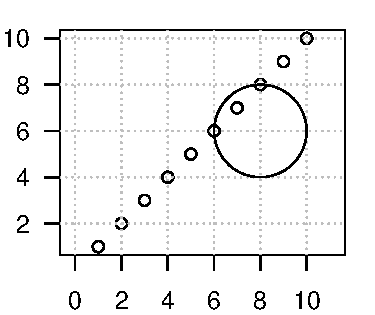
\includegraphics[width=0.4\textwidth]{./fig/circlebasics-1} 

}



\end{knitrout}
\end{frame}

%------------------------------------------------------------%

\begin{frame}[fragile]{Time to practice programming}
\begin{exercise}{Writing functions} %ex
Write a function that
\begin{enumerate}
  \item - draws a circle with a certain radius at user-specified locations of an existing plot (see last slide).
  \item - uses ellipsis to allow the user to customize the appearance
  \item - checks all the arguments and gives useful warnings if the wrong type of input is provided
  \item - has useful explanations for each argument (documentation)
  \item - has readable indentation, spacing and comments explaining the code
  \item Now let your neighbor use it without explaining how it is to be used (this should be inferred from the code and comments!)
  \item Use your neighbor's function with a vector to draw several circles at once. (unintended use?) What happens?
\end{enumerate}
\end{exercise}
\end{frame}

%------------------------------------------------------------%

\begin{frame}[fragile]
\begin{knitrout}\scriptsize
\definecolor{shadecolor}{rgb}{0.961, 0.961, 0.961}\color{fgcolor}\begin{kframe}
\begin{alltt}
\hlcom{# Small helper function drawing circles into existing graphics}
\hlcom{# Berry Boessenkool, berry-b@gmx.de, 2012}
\hlstd{circle} \hlkwb{<-} \hlkwa{function}\hlstd{(}
  \hlkwc{x}\hlstd{,} \hlcom{# x-coordinate of points, numeric value of length 1}
  \hlkwc{y}\hlstd{,} \hlcom{# ditto for y}
  \hlkwc{r}\hlstd{,} \hlcom{# radius of the circle, in the graphic's units}
  \hlkwc{locnum}\hlstd{=}\hlnum{100}\hlstd{,} \hlcom{# number of points on circle (more means smoother but slower)}
  \hlkwc{...}\hlstd{)} \hlcom{# Further Arguments passed to polygon, like col, border, lwd}
 \hlstd{\{}
 \hlcom{# input checking - only one circle can be drawn:}
 \hlkwa{if}\hlstd{(}\hlkwd{length}\hlstd{(x)} \hlopt{>}\hlnum{1} \hlopt{|} \hlkwd{length}\hlstd{(y)} \hlopt{>}\hlnum{1} \hlopt{|} \hlkwd{length}\hlstd{(r)} \hlopt{>}\hlnum{1} \hlopt{|} \hlkwd{length}\hlstd{(locnum)} \hlopt{>}\hlnum{1}\hlstd{)}
   \hlstd{\{}
   \hlkwd{warning}\hlstd{(}\hlstr{"Only the first element of the vectors is used."}\hlstd{)}
   \hlstd{x} \hlkwb{<-} \hlstd{x[}\hlnum{1}\hlstd{]; y} \hlkwb{<-} \hlstd{y[}\hlnum{1}\hlstd{]; r} \hlkwb{<-} \hlstd{r[}\hlnum{1}\hlstd{]; locnum} \hlkwb{<-} \hlstd{locnum[}\hlnum{1}\hlstd{]}
   \hlstd{\}}
 \hlcom{# input checking - is every value numeric?}
 \hlkwa{if}\hlstd{(}\hlopt{!}\hlkwd{is.numeric}\hlstd{(x))} \hlkwd{stop}\hlstd{(}\hlstr{"x must be numeric, not "}\hlstd{,} \hlkwd{class}\hlstd{(x))}
 \hlkwa{if}\hlstd{(}\hlopt{!}\hlkwd{is.numeric}\hlstd{(y))} \hlkwd{stop}\hlstd{(}\hlstr{"y must be numeric, not "}\hlstd{,} \hlkwd{class}\hlstd{(y))}
 \hlkwa{if}\hlstd{(}\hlopt{!}\hlkwd{is.numeric}\hlstd{(r))} \hlkwd{stop}\hlstd{(}\hlstr{"r must be numeric, not "}\hlstd{,} \hlkwd{class}\hlstd{(r))}
 \hlcom{# prepare circle line coordinates:}
 \hlstd{cx} \hlkwb{<-} \hlstd{x}\hlopt{+}\hlstd{r}\hlopt{*}\hlkwd{cos}\hlstd{(} \hlkwd{seq}\hlstd{(}\hlnum{0}\hlstd{,}\hlnum{2}\hlopt{*}\hlstd{pi,}\hlkwc{len}\hlstd{=locnum) )}
 \hlstd{cy} \hlkwb{<-} \hlstd{y}\hlopt{+}\hlstd{r}\hlopt{*}\hlkwd{sin}\hlstd{(} \hlkwd{seq}\hlstd{(}\hlnum{0}\hlstd{,}\hlnum{2}\hlopt{*}\hlstd{pi,}\hlkwc{len}\hlstd{=locnum) )}
 \hlkwd{polygon}\hlstd{(cx, cy, ...)} \hlcom{# actually draw it}
 \hlstd{\}}
\hlcom{# Note: if circles look like ellipsis, use plot(... asp=1)}
\end{alltt}
\end{kframe}
\end{knitrout}
\end{frame}

%------------------------------------------------------------%

\begin{frame}[fragile]{Solution for exercise \arabic{exercisecount} II: functions}
\begin{knitrout}
\definecolor{shadecolor}{rgb}{0.961, 0.961, 0.961}\color{fgcolor}\begin{kframe}
\begin{alltt}
\hlkwd{plot}\hlstd{(}\hlnum{1}\hlopt{:}\hlnum{20}\hlstd{,} \hlkwc{type}\hlstd{=}\hlstr{"n"}\hlstd{,} \hlkwc{asp}\hlstd{=}\hlnum{1}\hlstd{,} \hlkwc{cex}\hlstd{=}\hlnum{2}\hlstd{)}
\hlkwd{circle}\hlstd{(}\hlnum{5}\hlstd{,}\hlnum{5}\hlstd{,} \hlkwc{r}\hlstd{=}\hlnum{3}\hlstd{)}
\hlkwd{circle}\hlstd{(}\hlnum{15}\hlstd{,}\hlnum{10}\hlstd{,} \hlkwc{r}\hlstd{=}\hlnum{4}\hlstd{,} \hlkwc{locnum}\hlstd{=}\hlnum{12}\hlstd{,} \hlkwc{col}\hlstd{=}\hlnum{2}\hlstd{,} \hlkwc{border}\hlstd{=}\hlnum{4}\hlstd{,} \hlkwc{lwd}\hlstd{=}\hlnum{3}\hlstd{)}
\end{alltt}
\end{kframe}

{\centering 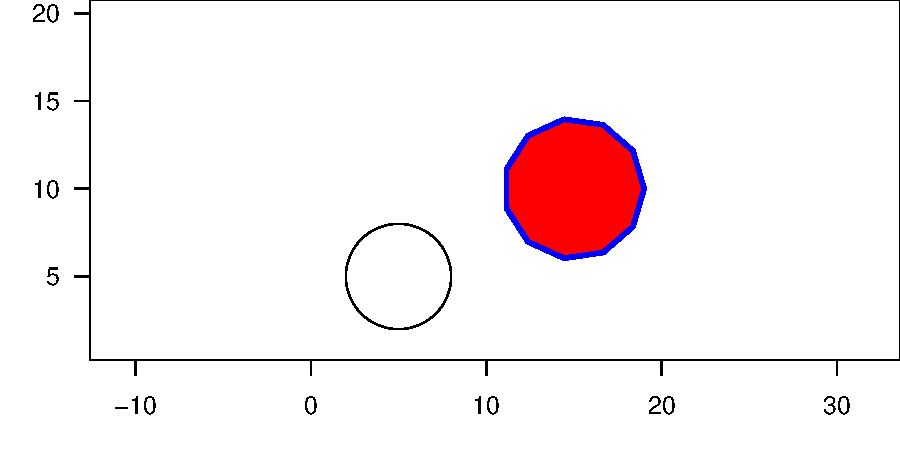
\includegraphics[width=\textwidth]{./fig/exfunsolb-1} 

}



\end{knitrout}
\end{frame}

%------------------------------------------------------------%

\begin{frame}[fragile]{Solution for exercise \arabic{exercisecount} III: functions}
\begin{knitrout}\scriptsize
\definecolor{shadecolor}{rgb}{0.961, 0.961, 0.961}\color{fgcolor}\begin{kframe}
\begin{alltt}
\hlcom{# can not be vectorized:}
\hlstd{x} \hlkwb{<-} \hlkwd{sample}\hlstd{(}\hlnum{1}\hlopt{:}\hlnum{20}\hlstd{,} \hlnum{15}\hlstd{) ;  y} \hlkwb{<-} \hlkwd{sample}\hlstd{(}\hlnum{1}\hlopt{:}\hlnum{20}\hlstd{,} \hlnum{15}\hlstd{) ; r} \hlkwb{<-} \hlkwd{runif}\hlstd{(}\hlnum{20}\hlstd{)}\hlopt{*}\hlnum{4}
\hlkwd{circle}\hlstd{(x,y,r,} \hlkwc{col}\hlstd{=}\hlkwd{rgb}\hlstd{(}\hlnum{1}\hlstd{,}\hlnum{0.5}\hlstd{,}\hlnum{0}\hlstd{,}\hlkwc{alpha}\hlstd{=}\hlnum{0.4}\hlstd{),} \hlkwc{border}\hlstd{=}\hlnum{NA}\hlstd{)}
\end{alltt}


{\ttfamily\noindent\color{warningcolor}{\#\# Warning in circle(x, y, r, col = rgb(1, 0.5, 0, alpha = 0.4), border = NA): Only the first element of the vectors is used.}}\begin{alltt}
\hlkwa{for}\hlstd{(i} \hlkwa{in} \hlnum{1}\hlopt{:}\hlnum{15}\hlstd{)} \hlkwd{circle}\hlstd{(x[i],y[i],r[i],} \hlkwc{col}\hlstd{=}\hlkwd{rgb}\hlstd{(}\hlnum{1}\hlstd{,}\hlnum{0.5}\hlstd{,}\hlnum{0}\hlstd{,}\hlkwc{alpha}\hlstd{=}\hlnum{0.4}\hlstd{),} \hlkwc{border}\hlstd{=}\hlnum{NA}\hlstd{)}
\end{alltt}
\end{kframe}

{\centering 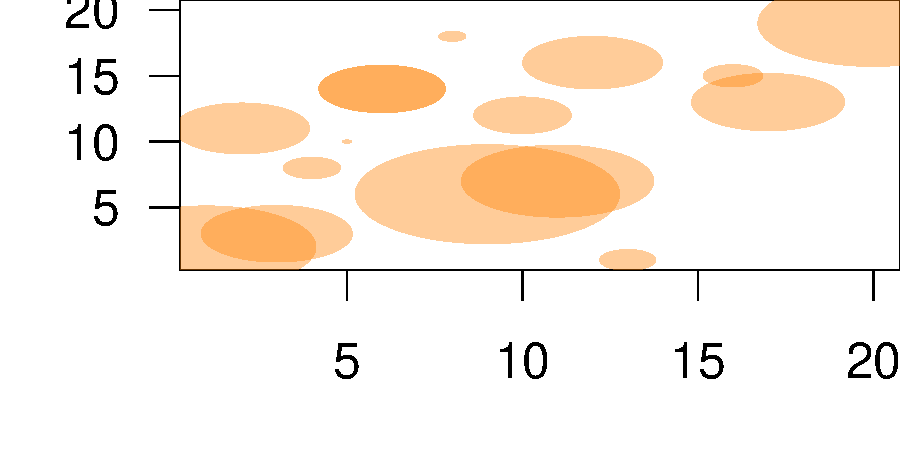
\includegraphics[width=0.65\textwidth]{./fig/exfunsolc-1} 

}



\end{knitrout}
\end{frame}

\iffalse % commenting out R packages section
%------------------------------------------------------------%

\section{Writing R packages}

%------------------------------------------------------------%

\begin{frame}{Why you should write R packages}
\pause
\begin{itemize}[<+->]
\item Collect your own functions in one place
\item Combine functions and documentation in the right way
\item Share code with others
\item Make your research reproducible !
\end{itemize}
\onslide<+->
\vspace{1em}
Good introduction at \datalinkText{packdev.R}
\end{frame}

\fi % commenting out R packages section
%------------------------------------------------------------%


\section{Debugging}

% ---------------------------

\begin{frame}[fragile]{Debugging}
\begin{itemize}[<+->]
\item Your code throws an error.
You didn't call the mentioned function.
Obviously, your code calls some function calling some function calling some function calling [you get the idea] which in the end creates an error.
To trace back this path, you can use \rcode{traceback()}.

\item Now that you know where the error originates from, you set \rcode{options(error=recover)}.
You run your code again, but this time R waits at the level creating an error.
You examine the environment within the function, play around with the objects and internal function code, until the bug has been fixed.
You have just debugged a function.

\item You want to step into the function you are developing at a specific point.
You add \rcode{browser()} at that point of the code.
You want to go line by line in one specific function. You set \rcode{debug(thatFunction)}.

\item You want to learn about lexical scoping (Where does R find variables?).\\
\small
\href{http://trestletech.com/2013/04/package-wide-variablescache-in-r-package/}{http://trestletech.com/2013/04/package-wide-variablescache-in-r-package/}
\href{http://adv-r.had.co.nz/Environments.html}{http://adv-r.had.co.nz/Environments.html}
\end{itemize}
\end{frame}

% ---------------------------

\begin{frame}[fragile]{Debugging: useful functions}
\begin{tabular}{ll}
\pause source("projectFuns.R") & execute complete file\\
\pause traceback() & find error source in sequence of function calls\\
\pause options(warn=2) & warnings to error. default 0\\
\pause browser() & go into function environment: \rcode{n}, \rcode{s}, \rcode{f}, \rcode{c}, \rcode{Q}\\
\pause \alert{options(error=recover)} & \alert{open interactive session where error occurred}\\
\pause debug(funct) & toggle linewise function execution\\
\pause undebug(funct) & after calling and fixing funct\\
\end{tabular}\\
\pause
\vspace{-0.5em}
\begin{knitrout}\footnotesize
\definecolor{shadecolor}{rgb}{0.961, 0.961, 0.961}\color{fgcolor}\begin{kframe}
\begin{alltt}
\hlkwa{if}\hlstd{(}\hlkwd{length}\hlstd{(input)}\hlopt{>}\hlnum{1}\hlstd{)} \hlkwd{stop}\hlstd{(}\hlstr{"length must be 1, not "}\hlstd{,} \hlkwd{length}\hlstd{(input))}
\end{alltt}
\end{kframe}
\end{knitrout}
\vspace{-1em}
\pause
\rcode{stop}: Interrupts function execution and gives error\\
\rcode{warning}: continues but gives warning\\
\rcode{message}: to inform instead of worry the user\\[1em]
\pause
\href{http://www.biostat.jhsph.edu/~rpeng/docs/R-debug-tools.pdf}{R. Peng (2002): Interactive Debugging Tools in R}\\
\href{https://www.stats.umanitoba.ca/files/statsweb/2011/03/debugging.pdf}{D. Murdoch (2010): Debugging in R}\\
\href{http://adv-r.had.co.nz/Exceptions-Debugging.html}{H. Wickham (2015): Advanced R: debugging}\\
Example: \href{https://www.r-bloggers.com/tracking-down-errors-in-r/}{Pete Werner Blog Post (2013)}
\end{frame}

%------------------------------------------------------------%

\begin{frame}[fragile]{Practice debugging, \datalinkText{lsc\_functions.R}}
\begin{exercise}{Debugging}
\begin{enumerate}
\item Load your package and the datasets. Correct the functions until\\
\rcode{lsc(calib\$P, calib\$Q, area=1.6)} returns the result below.
\item BONUS: commit each change to git.
\end{enumerate}
\end{exercise}

\begin{knitrout}
\definecolor{shadecolor}{rgb}{0.961, 0.961, 0.961}\color{fgcolor}

{\centering 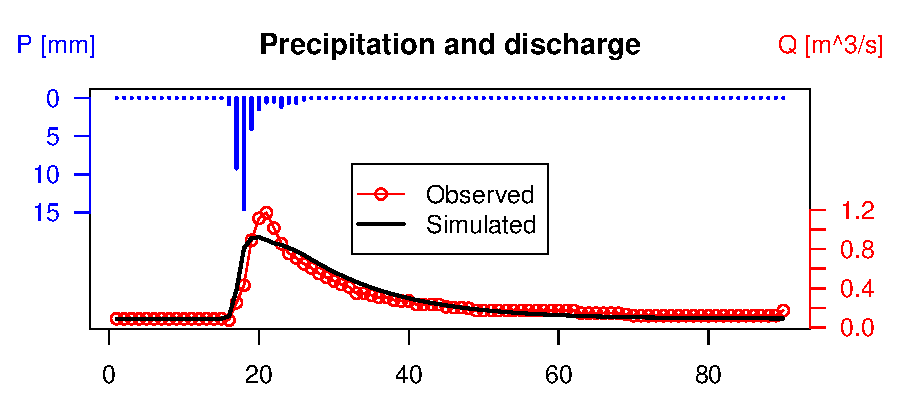
\includegraphics[width=\textwidth]{./fig/PQ_lsc-1} 

}



\end{knitrout}
\end{frame}

%------------------------------------------------------------%

\begin{frame}[fragile]{Solution for exercise \arabic{exercisecount}: Debugging}
\begin{itemize}
\item \rcode{stupid error you can easily remove} - traceback - find location of error - lsc\#73 - just comment it out
\item \rcode{harder to find but still stupid} - traceback - nse\#11 - ditto
\item \rcode{Error in plot: need finite 'ylim' value} - debug/browser/options(error=recover) - lsc\#105 - NAs in Q - range(Q, na.rm=TRUE) - also in other applicable locations
\item \rcode{There were 50 or more warnings} - come from rmse being called in optimization - add argument quietNA (or similar) to lsc that is passed to rmse in lsc\#79
\end{itemize}
\end{frame}

%------------------------------------------------------------%
%------------------------------------------------------------%
\section{Feedback}
%------------------------------------------------------------%
%------------------------------------------------------------%

\begin{frame}{Feedback}
\center{
Please fill out the feedback form at\\[1em]
\href{https://bit.ly/feedbackR}{bit.ly/feedbackR}\\[1em]
(it only takes a few minutes and helps to improve the course)\\[1em]
Thanks!\\[1em]
}
\end{frame}

%------------------------------------------------------------%
%------------------------------------------------------------%
\end{document}
%------------------------------------------------------------%
%------------------------------------------------------------%

